\documentclass[11pt,twoside]{article}
\usepackage{techrep-PFG-ic}
\usepackage[english]{babel}
\usepackage[utf8]{inputenc}
\usepackage{amsmath}
\usepackage{amssymb}
\usepackage{array}
\usepackage{caption}
\usepackage{float}
\usepackage{hyperref}
\usepackage{url}

\DeclareMathOperator*{\E}{\mathbb{E}}
\DeclareMathOperator*{\argmax}{\arg\!\max}

\newcommand{\subsubsubsection}[1]{\paragraph{#1}\mbox{}\\}
\setcounter{secnumdepth}{4}
\setcounter{tocdepth}{4}

\begin{document}

%%% PÁGINA DE CAPA %%%%%%%%%%%%%%%%%%%%%%%%%%%%%%%%%%%%%%%%%%%%%%%

% Número do relatório
\TRNumber{13} 

% DATA DE PUBLICAÇÃO (PARA A CAPA)
%
\TRYear{18}  % Dois dígitos apenas
\TRMonth{07} % Numérico, 01-12

% LISTA DE AUTORES PARA CAPA (sem afiliações).
\TRAuthor{Guilherme Bueno Andrade \and Andre Rodrigues Oliveira \and Zanoni Dias}

% TÍTULO PARA A CAPA (use \\ para forçar quebras de linha).
\TRTitle{Sorting Permutations by Reversals with Reinforcement Learning}

\TRMakeCover

\markboth{Andrade, Oliveira and Dias}{Sorting Permutations with RL}
\pagestyle{myheadings}

\title{Sorting Permutations by Reversals\\ with Reinforcement Learning}

\newcommand*\samethanks[1][\value{footnote}]{\footnotemark[#1]}
\author{Guilherme Bueno Andrade\thanks{gbuenoandrade@gmail.com} \and
Andre Rodrigues Oliveira\thanks{Institute of Computing, University of Campinas, Brazil.} \and Zanoni Dias\samethanks}

\date{}

\maketitle

%%%%%%%%%%%%%%%%%%%%%%%%%%%%%%%%%%%%%%%%%%%%%%%%%%%%%%%%%%%%%%%%%%%%%%

\begin{abstract} 

Finding the minimum number of mutations necessary for one genome to transform into another is a major problem in molecular biology. If genomes are represented as numeric permutations, this problem can be reduced to sorting such permutations using certain genome rearrangements operations, where, in this work, reversals operations are the main focus. We present two different techniques using reinforcement learning to address that. Our results show that this approach is competitive for permutations of size $n < 11$. However, as the permutations grow, converging gets trickier.

\end{abstract}

\section{Introduction}

Finding the minimum number of mutations necessary for one genome to transform into another using genome rearrangements, a concept usually referred to as \textit{distance} between genomes, is a major problem in molecular biology. Common operations are reversals. They happen when a fragment of the DNA filament gets reversed in the final replica. 

Formally, in this work we treat a genome of size $n$ as being equal to a permutation $p$ of integers from $0$ to $n - 1$. Also, we define the composition of permutations $p$ and $q$ as being $p \cdot q = (p_{q_0}\ p_{q_1}\ \ldots\ p_{q_{n-1}})$. In addition to that, we assume that a reversal operation $f_r(i,j)$ applied to permutation $p = (p_0\ \ldots\ p_{i-1}\ \underline{p_{i}\ \ldots\ p_{j}}\ \ldots\ p_{n-1})$ generates $p \cdot f_r(i,j) = (p_0\ \ldots\ p_{i-1}\ \underline{p_{j}\ \ldots\ p_{i}}\ \ldots\ p_{n-1})$.

Finally, as Phylogenetics (the study of evolutionary history and relationships between species) relies strongly on the Principle of Parsimony, the idea that, given a set of possible explanations for a fact, the simplest explanation is most likely to be correct ~\cite{parsimony}, the distance $d(p, q)$ between permutations $p$ and $q$ is the minimum number of operations needed to transform $p$ into $q$. 

Finding $d(p, q)$ is equivalent to the problem of finding the distance between some permutation $\alpha$ and the identity permutation $\iota$, where $\alpha = q^{-1} \cdot p$. That is the case because $d(p, q) = d(q^{-1} \cdot p, q^{-1} \cdot q) = d(\alpha, \iota)$. Furthermore, Caprara proved that finding $d$ is NP-hard~\cite{caprara1999sorting}. That being so, this work proposes using Reinforcement Learning to come up with a heuristic for finding $d(p, \iota)$ for any arbitrary permutation $p$.

In the next Section, we start by introducting several Reinforcement Learning ideas that were used during the project conception. Later, in Section \ref{section:expr}, we conclude by talking about implementation details and discussing our findings.

\section{Reinforcement Learning}

This section introduces the main ideas and concepts from Reinforcement Learning that have been explored during the implementation of the project. It starts by introducing basic ideas from the field, and ends talking about the algorithms which supported our agents.

\subsection{Overview}

Reinforcement Learning (RL), like other branches of Machine Learning, has been drawing a lot of attention from the community in recent years. Google DeepMind's AlphaGo victory over Lee Sedol~\cite{googlelee} - world champion of the game Go, is one out of many examples of recent astonishing applications of the technique. It is based on an agent learning how to accomplish a certain goal based on interactions with the environment.

RL can be thought of as a sequence of episodes. Each of which consists of the agent at an initial state $S_0$. Then, based on a policy $\pi$, where a policy is a function that maps states to actions, it takes an action $a$, ending up at state $S_1$ and receiving some reward $R_1$. This process keeps going until the agent reaches a terminal state. Its goal is to find a function $\pi*$, known as optimal policy, that maximizes the cumulative discounted reward at a given time step $t$:

\begin{gather}
	G(t) = \sum_{\tau = 0}^{\infty} \gamma ^ {\tau} R_{t + \tau + 1}
	,
\intertext{Where:}
	\begin{tabular}{>{$}r<{$}@{\ :\ }l}
		\gamma \in [0,1) & is a discount rate to highlight most likely short-term rewards
	\end{tabular}\nonumber
\end{gather}

\subsection{Exploitation vs. Exploration}
 
A major concern in RL is the exploitation/exploration trade-off. Exploration is about exploring new possibilities within the environment and finding out more information about it. Exploitation, on the other hand, is related to exploiting already known information so as to maximize the total reward. 

Initially, the agent has no other option but to randomly explore the environment; however, as it learns about its surroundings, it can fall into the trap of sticking to safe known actions and miss larger rewards that depend on exploring unknown states.

This work uses the Epsilon-greedy strategy to address that problem. It specifies an exploration rate $\epsilon$, which is set to 1 initially. This rate defines the ratio of the steps that will be done randomly. Before selecting an action, the agent generates a random number $x$. If $x > \epsilon$, then it will select the best known action (exploit); otherwise, it will select an action at random (explore). As the agent acquires more knowledge about the environment, $\epsilon$ is progressively reduced.

\subsection{Q-table and the Bellman Equation}

In value-based RL, the branch being considered in this work, the efforts are concentrated on maximizing the value function $V_\pi$. It tells the agent the expected cumulative discounted reward it will get if it is at state $s$ during time step $t$:

\begin{gather}
	V_\pi(s) = \mathbb{E}_{\pi} [G(t)\ |\ S_t = s]
	,
\intertext{Where:}
	\begin{tabular}{>{$}r<{$}@{\ :\ }l}
	\mathbb{E}_{\pi} & expected value given that policy $\pi$ is being followed
	\end{tabular}\nonumber
\end{gather}

 $V_\pi$ can be generalized so as to also consider the action $a$ taken at time step $t$, which is known as Q-table:

\begin{equation} \label{qtable}
	Q^\pi(s, a) = \mathbb{E}_{\pi} [G(t)\ |\ S_t = s,\ A_t = a]
\end{equation}

The previous definition is convenient because it allows the agent to pick the best action that can be performed from state $s$ by simply finding $\operatorname*{arg\,max}_{a} Q^\pi(s,a)$.

Furthermore, $Q$ can be expressed in terms of itself. An expression known as the Bellman Equation~\cite{sutton}:

\begin{gather}\label{bellman}
	Q^\pi(s, a) = \mathbb{E}_{\pi} [R_{t+1} + \gamma \sum_{a'} Q^\pi(s', a')]
	,
\intertext{Where:}
	\begin{tabular}{>{$}r<{$}@{\ :\ }l}
		s' & is the state reached after action $a$ is taken from state $s$ \\
		a' & is an action that can be taken from $s'$
	\end{tabular}\nonumber
\end{gather}

The above equation can be used alongside dynamic programming to develop iterative approaches to solve the problem~\cite{sutton}.

If one can calculate the Q-table from Equation \ref{qtable}, they could trivially come up with a great policy. At each state $s$, the agent should simply be greedy and select the action $a$ that maximizes $Q^\pi(s, a)$. As mentioned above, finding the Q-table can be easily done with dynamic programming.

However, as the number of states grows, dynamic programming and other iterative approaches become infeasible due to space and time limitations. Fortunately, it turns out that the Q-table can be approximated instead of having its exact values determined, and it will still produce great results~\cite{dp_approx}. This work tries to achieve that using both linear regression and deep neural networks.

\subsection{Monte Carlo and Temporal Difference Learning}

In Monte Carlo Approaches, the agent plays an entire episode, keeping track of the rewards received at each time step so it can calculate the cumulative discounted reward. After that, it updates the value function for each visited stated based on the expression~\cite{sutton}:

\begin{gather}
	V(S_t) \leftarrow V(S_t) + \alpha (G(t) - V(S_t))
	,
\intertext{Where:}
	\begin{tabular}{>{$}r<{$}@{\ :\ }l}
		\alpha & is the learning rate
	\end{tabular}\nonumber
\end{gather}

Therefore, the agent only learns after an entire episode has been played. In Temporal Difference Learning, on the other hand, the value of $V$ is updated after each time step. At time $t+1$, the observations made during time $t$ are already being considered. In its simplest form, the method is called TD(0) or 1-step TD, and its update equation is as follows:

\begin{equation} \label{td0}
	V(S_t) \leftarrow V(S_t) + \alpha (R_{t+1} + \gamma V(S_{t+1}) - V(S_t))
\end{equation}

The right-hand side of the previous equation is referred to as the TD(0) error.

TD(0) is biased as it relies on information from a single time step to perform its updates. It does not take into account the fact that the action that caused a reward might have happened several time steps earlier, which can lead to slow convergence~\cite{tdlambda}. Monte Carlo methods, although not biased, have a lot of variance since they use the rewards of an entire episode in order to perform updates~\cite{tdlambda}.

To overcome that, from Equation \ref{td0}, we can define the 1-step return, $G_t^{(1)} = R_{t+1} + \gamma V(S_{t+1})$. We can extend the concept further to 2-step return, $G_t^{(2)} = R_{t+1} + \gamma R_{t+2} + \gamma^2 V(S_{t+2})$, and, generically, to, $G_t^{(n)} = R_{t+1} + \gamma R_{t+2} + \ldots + \gamma^n V(S_{t+n})$. 

TD-Lambda methods use a mathematical trick to average all the possible n-step returns into a single one. This is done by introducing a factor $\lambda \in [0, 1]$ and weighting the nth-return with $\gamma^{n-1}$. It can be shown that when $\lambda = 0$, the method is equivalent to TD(0), and when $\lambda = 1$, equivalent to Monte Carlo~\cite{dp_approx}. So, intuitively, by setting $0 < \lambda < 1$, we can get a mixture of both methods.

\subsection{Q-learning}

Q-learning is another technique based on Temporal Difference Learning to learn the Q-table. The main difference between it and the previous shown techniques is that Q-learning is off-policy, while TD(0) and TD-Lambda are on-policy~\cite{sutton}. This is reflected in its update equation, derived from the Bellman Equation~\cite{qlearning}:

\begin{equation} \label{qlearning}
	Q(s, a) \leftarrow Q(s, a) + \alpha (R_{t+1} + \gamma \max_{a'} Q(s', a') - Q(s,a))
\end{equation}

The fact that there is no constraint acting upon action $a'$, only that it must optimizes $Q$, makes it an off-policy method~\cite{qlearning}.

\subsubsection{Deep Q-learning}

In order to approximate the Q-table to make using it feasible even when the number of states is very large, since Google AlphaGo's paper~\cite{alphago}, it has become common the use of deep neural networks. Even though standard Q-learning is proven to converge when there are finite states and each pair state-action is presented repeatedly~\cite{convergence_qlearning}, the same proof does not hold when neural networks are being used to calculate $Q$. To face with this issue, this work makes use of several ideas found in the literature~\cite{replay} to stabilize the training. They are presented in the following subsections.

\subsubsection{Experience Replay}\label{experience}

During each step of an episode, our estimation can be shifted according to Equation \ref{qlearning}. It is reasonable to think that as more truth is being introduced into the system, it will eventually converge; however, this is often not true. One of the reasons is that samples arrive in order they are experienced and as such are highly correlated. Also, by throwing away our samples immediately after we use it, we are not extracting all the knowledge they carry.

Experience replay address that by storing samples into a queue, and, during each learning step, it samples a random batch and performs gradient descend on it. As samples get old, they are gradually discarded.

\subsubsection{Target Network}

The points $Q(s, a)$ and $Q(s', a')$ in Equation \ref{qlearning} are very close together as $s'$ is a state reachable from $s$. That being so, updates to one of them influence the other, which in turn can lead to instabilities.

To overcome that, a second network, called target network, can be used to provide more stable $\widetilde{Q}$ values. This second network is a mere copy of the first one; however, it does not get updated every simulation step. Instead, it stays frozen in time, and only after several steps it is updated by copying the weights from the first network. The introduction of the target network changes our update equation to the following:

\begin{equation} \label{new_qlearning}
	Q(s, a) \leftarrow Q(s, a) + \alpha (R_{t+1} + \gamma \max_{a'}\widetilde{Q}(s', a') - Q(s,a))
\end{equation}

\subsubsection{Double Learning}\label{double_learning}

Due to the $\max$ term presented in both equations \ref{qlearning} and \ref{new_qlearning}, the approximation tends to overestimate the Q function value, which can severely impact on stability of the algorithm~\cite{overestimation}. A solution proposed by Hado van Hasselt (2010)~\cite{doubleq2010}, called Double Learning, consists of using two Q functions, $Q_1$ and $Q_2$, that are independently learned. One function is then used to determine the maximizing action and second to estimate its value. As we are already making use of two different networks, Hado van Hasselt's approach can be easily introduced to the update Equation \ref{new_qlearning}. Its augmented version is as follows:

\begin{equation}\label{double_equation}
	Q(s, a) \leftarrow Q(s, a) + \alpha (R_{t+1} + \gamma \widetilde{Q}(s', \argmax_{a'}{Q(s', a')}) - Q(s,a))
\end{equation}

\section{Experiment}\label{section:expr}

Initially, in Section \ref{state_rep}, we discuss different ways to represent the permutations so we can use function approximation techniques. Later, in Section \ref{arch}, we talk about the agents' architecture and about a technique that was used to speed up the convergence in Section \ref{speed_conv}. Lastly, we present and discuss our results and conclusions.

\subsection{Modeling}

The agents were implemented so as to perform not only reversals, but also another important genome rearrangement: transposition; however, due to limited computer resources available, we decided later to limit our agents to only perform reversals to make training faster. Their goal was to reach the identity permutation $\iota$ while maximizing total reward. 

\subsubsection{State Representation}\label{state_rep}

Three different state representations were considered. They are as follows.

\begin{itemize}
	\item \textit{One-Hot Encoding}: Each number is treated as a category. By doing so, each $p$ is mapped to a matrix $m$, where $m_{ij} = 1$ if $p_i = j$, and $0$ otherwise. 
	\item \textit{Min-Max Normalization}: $p$ is mapped to an array $v$, where $v_i = p_i / (|p| - 1)$.
	\item \textit{Permutation Characterization}: $p$ is mapped to an array $v$ of $30$ features, where the features are the ones described in the work by Silva, Oliveira, and Dias~\cite{flavio}.
\end{itemize}

\subsubsection{Proposed Architecture}\label{arch}

The experiment was based on two different architectures. The first one consisted of a Double Deep Q-Network (DDQN), with a main network and a secondary target network. Also, it included experience replay (see Section \ref{experience}) and double learning (see Section \ref{double_learning}) optimizations.

Both main and secondary networks used the following architecture:

\begin{table}[H]
	\begin{center}
		\begin{tabular}{|c|c|c|c|} 
			\hline
			Layer & Number of Units & Activation & Type \\
			\hline\hline
			Input layer & - & Linear & - \\ 
			\hline
			Hidden layer 1 & 256 & ReLU & Fully-connected\\
			\hline
			Hidden layer 2 & 256 & ReLU & Fully-connected\\
			\hline
			Output layer & $|$Actions$|$ & Linear & Fully-connected\\
			\hline
		\end{tabular}
		\caption{Main and secondary networks architecture}
	\end{center}
\end{table}

Furthermore, after tuning, the hyperparameters selected were as follows:

\begin{table}[H]
	\begin{center}
		\begin{tabular}{|c |c|} 
			\hline
			Hyperparameter & Value \\
			\hline\hline
			$\gamma$ & $0.99$ \\
			$\alpha$ & $0.001$ \\
			$|$Batch$|$ & $32$ \\
			$\epsilon_{min}$ & $0.1$ \\
			$\epsilon_{decay}$ & $0.993$ \\
			$|$Replay queue$|$ & 2000 \\
			Loss & logcosh \\
			Optimizer & Adam \\
			Step reward & $-1$ \\
			\hline
		\end{tabular}
		\caption{Hyperparameters used in the DDQN}
	\end{center}
\end{table}

Nevertheless, we tried a second approach. An agent based on the TD-Lambda algorithm was also built. In order to approximate the Q-table, it relied on a much simpler linear regressor. Also, since $Q$ is highly nonlinear (see Equation \ref{bellman}), the radial basis function kernel was used as a pre-processing step. The agent's hyperparameters were the following:

\begin{table}[H]
	\begin{center}
		\begin{tabular}{|c |c|} 
			\hline
			Hyperparameter & Value \\
			\hline\hline
			$\gamma$ & $0.999$ \\
			$\alpha$ & $0.01$ \\
			$\lambda$ & $0.25$ \\
			$\epsilon_{min}$ & $0.05$ \\
			$\epsilon_{decay}$ & $0.99$ \\
			RBF Components & $4$ \\
			RBF $\gamma$ array & $[5.0, 2.0, 1.0, 0.5]$ \\
			Step reward & $-1$ \\
			\hline
		\end{tabular}
		\caption{Hyperparameters used to implement TD-Lambda}
	\end{center}
\end{table}

\subsubsection{Speeding up the Convergence}\label{speed_conv}

During our initial tests, the Q-table took a long time to converge to optimal values. Being that the case, several techniques were tried so as to decrease training time. The one that seemed more promising is described below:

\begin{itemize}
	\item \textit{Greedy Pre-Training}: Kececioglu and Sankoff~\cite{Kececioglu1995} presented a 2-approximation for sorting a permutation using reversals, its output is represented below:

	\begin{gather}\label{greedy}
		\widetilde{d}(p) = (p,\ a(p),\ a'(a(p)),\ \ldots,\ \iota)
		,
	\intertext{Where:}
		\begin{tabular}{>{$}r<{$}@{\ :\ }l}
			a & is the resultant permutation after applying action $a$ on $p$ \\
			\iota & is the identity permutation
		\end{tabular}\nonumber
	\end{gather}

	From Equation \ref{greedy}, let $\hat{V}$:
	\begin{equation}
		\hat{V}(s) = (\gamma^{|\widetilde{d}(s)|} - 1) / (\gamma - 1)
	\end{equation}

	Furthermore, we can define function $\hat{Q}$, which can be shown to be lower bound on $Q$:

	\begin{gather}
		\hat{Q}(s, a) = -1 + \gamma \hat{V}(s')
		,
	\intertext{Where:}
		\begin{tabular}{>{$}r<{$}@{\ :\ }l}
			s' & is the state reached by taking action $a$ at state $s$
		\end{tabular}\nonumber
	\end{gather}

	Having defined those, we can talk about our pre-training strategy. It consisted of partially fitting our neural network and linear regressor to function $\hat{Q}$ before start learning from proper episodes.

\end{itemize}

\subsection{Results and Discussion}

The models were trained experiencing $10000$ episodes, each of which had $S_0$ set to a random permutation of size $n = 10$ using NumPy's random permutation generator~\cite{numpy_permut} (see Figure \ref{chart:dist_evolution}). After that, in order for the models to effectively sort a permutation $p$, the exploration rate $\epsilon$ was kept constant and equal to $0.2$, and then the models were run for another $100$ episodes, where $S_0$ was always equal to $p$. The best score among those simulations was considered the model's answer $\hat{d}(p, \iota)$. Finally, we used Kececioglu and Sankoff's greedy algorithm output $|\widetilde{d}(p)|$ and ours for $1000$ random permutations as a way to measure the model's performance.

As we can see in Table \ref{table:results}, one-hot encoding state representation is slightly better than our Min-Max approach. The former beat Kececioglu and Sankoff's in 28.0\% of the simulations, while the latter only in 21.7\%. Nonetheless, investigating more effective representations so as to lead to better generalizations is a pending task. Also, we did not manage to reach convergence using either DDQN and Permutation Characterization or the TD-Lambda agent for permutations of size $n > 8$. Regarding our best RL archicture - DDQN and One-Hot Encoding, it consistently outperformed Kececioglu and Sankoff's. However, converging starts getting tricky and time-consuming as $n$ gets bigger. So, it is still early to define our approach as being \textit{practical}.

\begin{table}[H]
	\begin{center}
		\begin{tabular}{|c|c|c|c|c|}
			\hline
			Configuration & $\hat{d} < |\widetilde{d}|$ & $\hat{d} = |\widetilde{d}|$ & $\hat{d} > |\widetilde{d}|$ & Avg $\hat{d}/d$\\
			\hline\hline
			\textbf{DDQN and One-Hot Encoding} & \textbf{28.0\%} & \textbf{64.7\%} & \textbf{7.3\%} & \textbf{1.0255}\\
			DDQN and Min-Max Normalization & 21.7\% & 61.2\% & 17.1\% & 1.0574\\
			DDQN and Permutation Characterization & 0.0\% & 0.0\% & 100.0\% & $\infty$\\
			TD-Lambda & 0.0\% & 0.0\% & 100.0\% & $\infty$\\
			\hline
		\end{tabular}
		\caption{Summary of the performance of different model configurations}
	\label{table:results}
	\end{center}
\end{table}


\begin{figure}[H]
	\begin{center}
		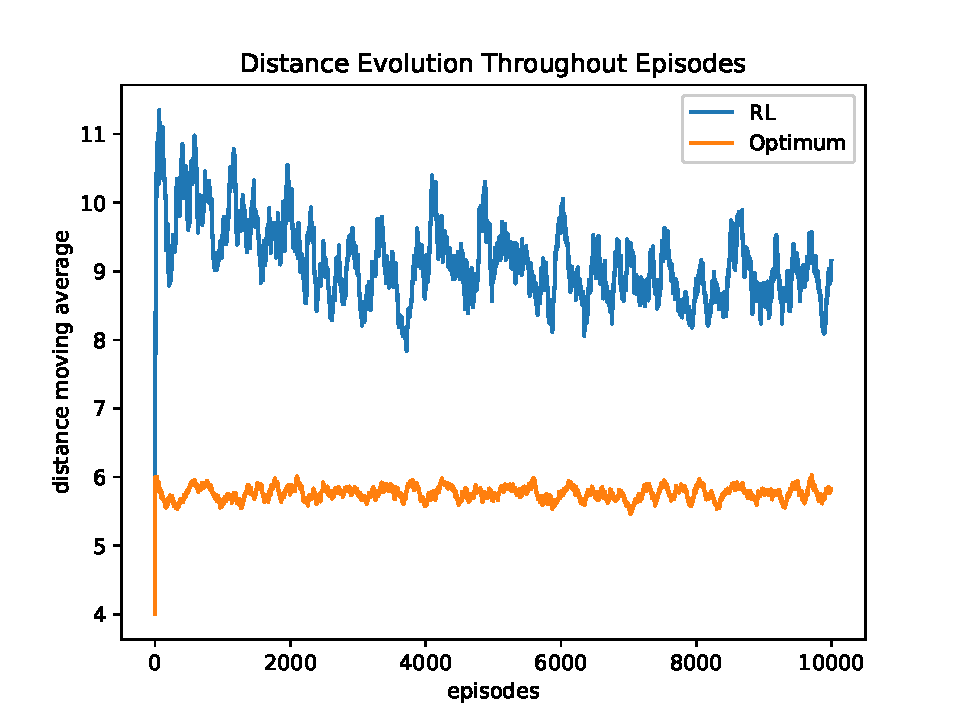
\includegraphics[scale=0.8]{charts/dist_evolution.pdf}
		\caption{Distance estimation evolution for DDQN and One-Hot Encoding}
		\label{chart:dist_evolution}
	\end{center}
\end{figure}

\subsection{Conclusions}

This work involved building different RL agents to sort permutations by reversals. Interesting results were obtained for small permutations, but performance was a bottleneck when they got bigger. Future work could try to address that by using distributed deep Q-learning methods~\cite{dist_dqnn1, dist_dqnn2} and considering recent findings related to large discrete action spaces~\cite{large_space}.

\bibliographystyle{abbrv}
\bibliography{main}

\end{document}
